\documentclass[12pt,a4paper]{article}

\usepackage[utf8]{inputenc}
\usepackage[T1]{fontenc}
\usepackage[brazil]{babel}
\usepackage[a4paper,margin=2.5cm]{geometry}
\usepackage{lmodern}
\usepackage{microtype}
\usepackage{graphicx}
\usepackage{xcolor}
\usepackage{booktabs}
\usepackage{tabularx}
\usepackage{array}
\usepackage{longtable}
\usepackage{caption}
\usepackage{listings}
\usepackage{hyperref}
\usepackage{enumitem}
\usepackage{fancyhdr}
\usepackage{titlesec}
\usepackage{amsmath,amssymb}
\usepackage{multirow}

\definecolor{spotgreen}{HTML}{1DB954}
\definecolor{lightgray}{HTML}{F5F5F5}
\definecolor{darkgray}{HTML}{333333}
\definecolor{codebg}{HTML}{FAFAFA}

\hypersetup{
  colorlinks=true,
  linkcolor=spotgreen!70!black,
  citecolor=spotgreen!70!black,
  urlcolor=spotgreen!70!black,
  pdftitle={Relatorio de Analise de Dados - Spotify Mobile IHC},
  pdfauthor={Equipe 01 - IHC 2026/1}
}

\titleformat{\section}{\Large\bfseries\color{darkgray}}{\thesection.}{0.6em}{}
\titleformat{\subsection}{\large\bfseries\color{darkgray}}{\thesubsection}{0.5em}{}

\pagestyle{fancy}
\fancyhf{}
\fancyhead[L]{\small IHC 2026/1 -- Equipe 01}
\fancyhead[R]{\small Spotify Mobile -- Análise de Dados}
\fancyfoot[C]{\thepage}
\renewcommand{\headrulewidth}{0.4pt}

\lstdefinestyle{pystyle}{
  language=Python,
  backgroundcolor=\color{codebg},
  basicstyle=\ttfamily\footnotesize,
  keywordstyle=\color{spotgreen!60!black}\bfseries,
  commentstyle=\color{gray}\itshape,
  stringstyle=\color{red!60!black},
  numbers=left,
  numberstyle=\tiny\color{gray},
  numbersep=8pt,
  breaklines=true,
  showstringspaces=false,
  frame=single,
  rulecolor=\color{gray!50},
  framesep=4pt,
  xleftmargin=14pt,
  tabsize=2,
}

\newcolumntype{Y}{>{\raggedright\arraybackslash}X}
\newcolumntype{R}{>{\raggedleft\arraybackslash}X}

\begin{document}

% =================== CAPA ===================
\begin{titlepage}
\centering
\vspace*{1.5cm}
{\Large\textbf{Universidade de Brasília}}\\[0.3cm]
{\large Departamento de Ciência da Computação}\\[0.3cm]
{\large Disciplina de Interação Humano-Computador --- 2026/1}\\[2.5cm]

{\color{spotgreen}\rule{\linewidth}{2pt}}\\[0.8cm]
{\huge\bfseries Análise de Dados de Avaliação de Usabilidade}\\[0.4cm]
{\Large Aplicativo Spotify Mobile (iOS / Android)}\\[0.4cm]
{\color{spotgreen}\rule{\linewidth}{2pt}}\\[1.5cm]

{\large Trabalho 2 --- Território n.\,04 (Análise de Dados)}\\[2cm]

\begin{tabular}{l}
\textbf{Equipe 01}\\[0.2cm]
Filipe Brito\\
Paulo Victor\\
João Vitor\\
Renan Câmara\\
Vitor Marconi\\
\end{tabular}

\vfill
{\large Professor: Sergio Freitas}\\[0.3cm]
{\large Brasília --- \today}
\end{titlepage}

% =================== RESUMO ===================
\section*{Resumo}
Este relatório apresenta a análise estatística dos resultados de um questionário de
avaliação de usabilidade do aplicativo \textbf{Spotify Mobile}, aplicado entre 31 de março
e abril de 2026 com $n = 86$ respondentes válidos. O instrumento, ancorado nas \textbf{10
Heurísticas de Nielsen}, mediu cinco dimensões previamente identificadas como violações
candidatas no Trabalho 1: \emph{Controle e Liberdade do Usuário} (H3), \emph{Consistência
e Padrões} (H4), \emph{Prevenção de Erros} (H5), \emph{Flexibilidade e Eficiência} (H7)
e \emph{Estética e Design Minimalista} (H8). O pipeline de análise segue exatamente o
modelo do professor (Território~n.\,04 e \texttt{exemplo.R}): estatística descritiva,
Alpha de Cronbach, Correlação de Pearson e Regras de Associação (Apriori).
Os resultados confirmam fortemente as hipóteses sobre \textbf{H7} e \textbf{H8},
parcialmente as de \textbf{H3} e \textbf{H5}, e não confirmam \textbf{H4} no agregado.
Identificam-se ainda \textbf{seis pontos de redesign} com evidência empírica robusta,
que pautam o protótipo de melhoria.

\vspace{0.5cm}\noindent
\textbf{Palavras-chave:} IHC, usabilidade, Heurísticas de Nielsen, Spotify, Alpha de
Cronbach, Apriori.

\tableofcontents
\newpage

% =================== 1. INTRODUÇÃO ===================
\section{Introdução e Contexto}
\label{sec:intro}

O Spotify é o serviço de \emph{streaming} de música mais utilizado no mundo, com
72\,\% das sessões ocorrendo em dispositivos móveis. Apesar disso, levantamentos prévios
realizados no \textbf{Trabalho 1} indicaram 54{,}54\,\% de insatisfação em mais de 60 mil
\emph{reviews} da Google Play Store e nota 1.6/5 no Trustpilot, sugerindo problemas
sistemáticos de experiência. A partir de análise heurística e de \emph{reviews}, o grupo
formulou cinco hipóteses de violação a serem testadas empiricamente:

\begin{itemize}[leftmargin=*, itemsep=2pt]
  \item \textbf{H3} --- Controle e Liberdade do Usuário;
  \item \textbf{H4} --- Consistência e Padrões;
  \item \textbf{H5} --- Prevenção de Erros;
  \item \textbf{H7} --- Flexibilidade e Eficiência de Uso;
  \item \textbf{H8} --- Design Estético e Minimalista.
\end{itemize}

O presente relatório descreve a \textbf{análise quantitativa e qualitativa} dos
dados coletados via questionário Likert (1--5), avalia o instrumento, identifica
relações entre dimensões e propõe melhorias diretamente acionáveis para o protótipo
de redesign.

% =================== 2. METODOLOGIA ===================
\section{Metodologia}
\label{sec:metod}

\subsection{Instrumento}
O questionário (versão \texttt{questionario\_spotify\_v2.pdf}) é composto por:
\begin{itemize}[leftmargin=*, itemsep=2pt]
  \item TCLE e item filtro de uso prévio;
  \item Cinco questões demográficas (faixa etária, escolaridade, frequência de uso,
        horas semanais e tipo de conta);
  \item \textbf{24 itens Likert} (1 = discordo totalmente; 5 = concordo totalmente),
        distribuídos em cinco blocos de cinco itens correspondentes às heurísticas
        H3, H4, H5, H7 e H8 (o bloco H8 possui quatro itens analisáveis no
        \textit{export} recebido);
  \item Três perguntas abertas (\emph{o que mais agrada/incomoda}; \emph{situações de
        confusão}; \emph{uma única mudança}).
\end{itemize}

\subsection{Coleta e Limpeza}
O formulário foi distribuído via Microsoft Forms, totalizando \textbf{90 respostas brutas}.
Após aplicar critérios de inclusão (consentimento + uso prévio do aplicativo),
restaram \textbf{86 respondentes válidos}. A Tabela~\ref{tab:perfil} traz o perfil
demográfico final.

\begin{table}[h]
\centering
\caption{Perfil demográfico da amostra válida ($n = 86$)}
\label{tab:perfil}
\small
\begin{tabularx}{\linewidth}{Y Y R}
\toprule
\textbf{Variável} & \textbf{Categoria predominante} & \textbf{\%}\\
\midrule
Faixa etária        & 18 a 24 anos                & 66{,}3\,\%\\
Escolaridade        & Superior cursando           & 62{,}8\,\%\\
Frequência de uso   & Todos os dias (ou quase)    & 74{,}4\,\%\\
Horas/semana        & De 1 a 5 horas              & 44{,}2\,\%\\
Tipo de conta       & Premium (Pago)              & 80{,}2\,\%\\
\bottomrule
\end{tabularx}
\end{table}

\subsection{Pipeline de Análise (Território n.\,04)}
Seguimos exatamente a sequência metodológica recomendada pelo professor Sergio Freitas
e exemplificada no \texttt{exemplo.R}:

\begin{enumerate}[label=\textbf{\arabic*.}, leftmargin=*, itemsep=2pt]
  \item \textbf{Carga e preparação} --- CSV com separador ``;'', tipos numéricos garantidos.
  \item \textbf{Estatística descritiva} --- média, desvio padrão, mediana e distribuição
        percentual por item e por bloco.
  \item \textbf{Confiabilidade (Alpha de Cronbach)} --- limiar do professor
        $\alpha > 0{,}7$ indica instrumento adequado.
  \item \textbf{Similaridade (Correlação de Pearson)} --- com tratamento de \emph{NA}
        por \texttt{pairwise.complete.obs}; faixas de interpretação: $|r| < 0{,}3$
        desprezível; $0{,}3$--$0{,}5$ fraca; $0{,}5$--$0{,}7$ moderada; $0{,}7$--$0{,}9$
        forte; $> 0{,}9$ muito forte.
  \item \textbf{Regras de Associação (Apriori)} --- discretização Likert
        ($1{-}2 = \textit{Baixo};\ 3 = \textit{Neutro};\ 4{-}5 = \textit{Alto}$) e
        extração de regras com suporte, confiança e \emph{lift}.
\end{enumerate}

\subsection{Implementação}
O pipeline original é escrito em R (bibliotecas \texttt{psychometric} e \texttt{arules}).
Por conveniência operacional, foi \textbf{reimplementado em Python} com NumPy/Pandas,
preservando os mesmos cálculos e limiares de interpretação. As fórmulas centrais são:

\paragraph{Alpha de Cronbach}
\[
\alpha \;=\; \frac{k}{k-1}\left(1 - \frac{\sum_{i=1}^{k}\sigma^{2}_{i}}{\sigma^{2}_{T}}\right)
\]
onde $k$ é o número de itens, $\sigma^{2}_{i}$ a variância de cada item e $\sigma^{2}_{T}$
a variância da soma dos itens. Adotamos \emph{listwise deletion} (mesmo comportamento
de \texttt{psychometric::alpha}).

\paragraph{Correlação de Pearson}
\[
r_{xy} = \frac{\sum_{i=1}^{n}(x_i - \bar{x})(y_i - \bar{y})}
{\sqrt{\sum_{i=1}^{n}(x_i - \bar{x})^{2}} \cdot \sqrt{\sum_{i=1}^{n}(y_i - \bar{y})^{2}}}
\]
calculado par a par (\texttt{pairwise.complete.obs}), preservando o máximo de respondentes.

\paragraph{Apriori (regras de associação)}
Suporte $\text{sup}(X) = |T_X|/|T|$, confiança
$\text{conf}(X \Rightarrow Y) = \text{sup}(X \cup Y)/\text{sup}(X)$,
e \emph{lift} $= \text{conf}/\text{sup}(Y)$. \emph{Lift} $>1$ indica associação
positiva entre os itens.

\subsection{Trecho central do código (Python)}
A Listagem~\ref{lst:cronbach} mostra a implementação de Cronbach e Apriori (excerto):

\begin{lstlisting}[style=pystyle, caption={Núcleo do pipeline (\texttt{analise.py}).}, label=lst:cronbach]
def cronbach_alpha(d):
    d = d.dropna(how='any')          # listwise deletion
    k = d.shape[1]
    var_items = d.var(axis=0, ddof=1).sum()
    var_total = d.sum(axis=1).var(ddof=1)
    return (k/(k-1)) * (1 - var_items/var_total)

def discretize(v):
    if pd.isna(v): return None
    if v <= 2: return 'Baixo'
    if v == 3: return 'Neutro'
    return 'Alto'

# Apriori: itens 1-, 2-, 3-itemsets que satisfacam min_sup,
# regras (lhs => rhs) com confianca >= min_conf, ordenadas por lift.
\end{lstlisting}

O script completo (\texttt{analise.py}) e a versão em R (\texttt{analise.R}, espelhando
o \texttt{exemplo.R}) estão disponíveis no diretório \texttt{docs/analise/}.

% =================== 3. RESULTADOS ===================
\section{Resultados}
\label{sec:resultados}

\subsection{Visão Geral por Bloco}
A Figura~\ref{fig:scores} apresenta o score médio de cada bloco com erro padrão
da média e os limiares de leitura. Nenhum bloco está abaixo do ponto neutro;
H4 é o melhor, H5 o pior.

\begin{figure}[h]
\centering
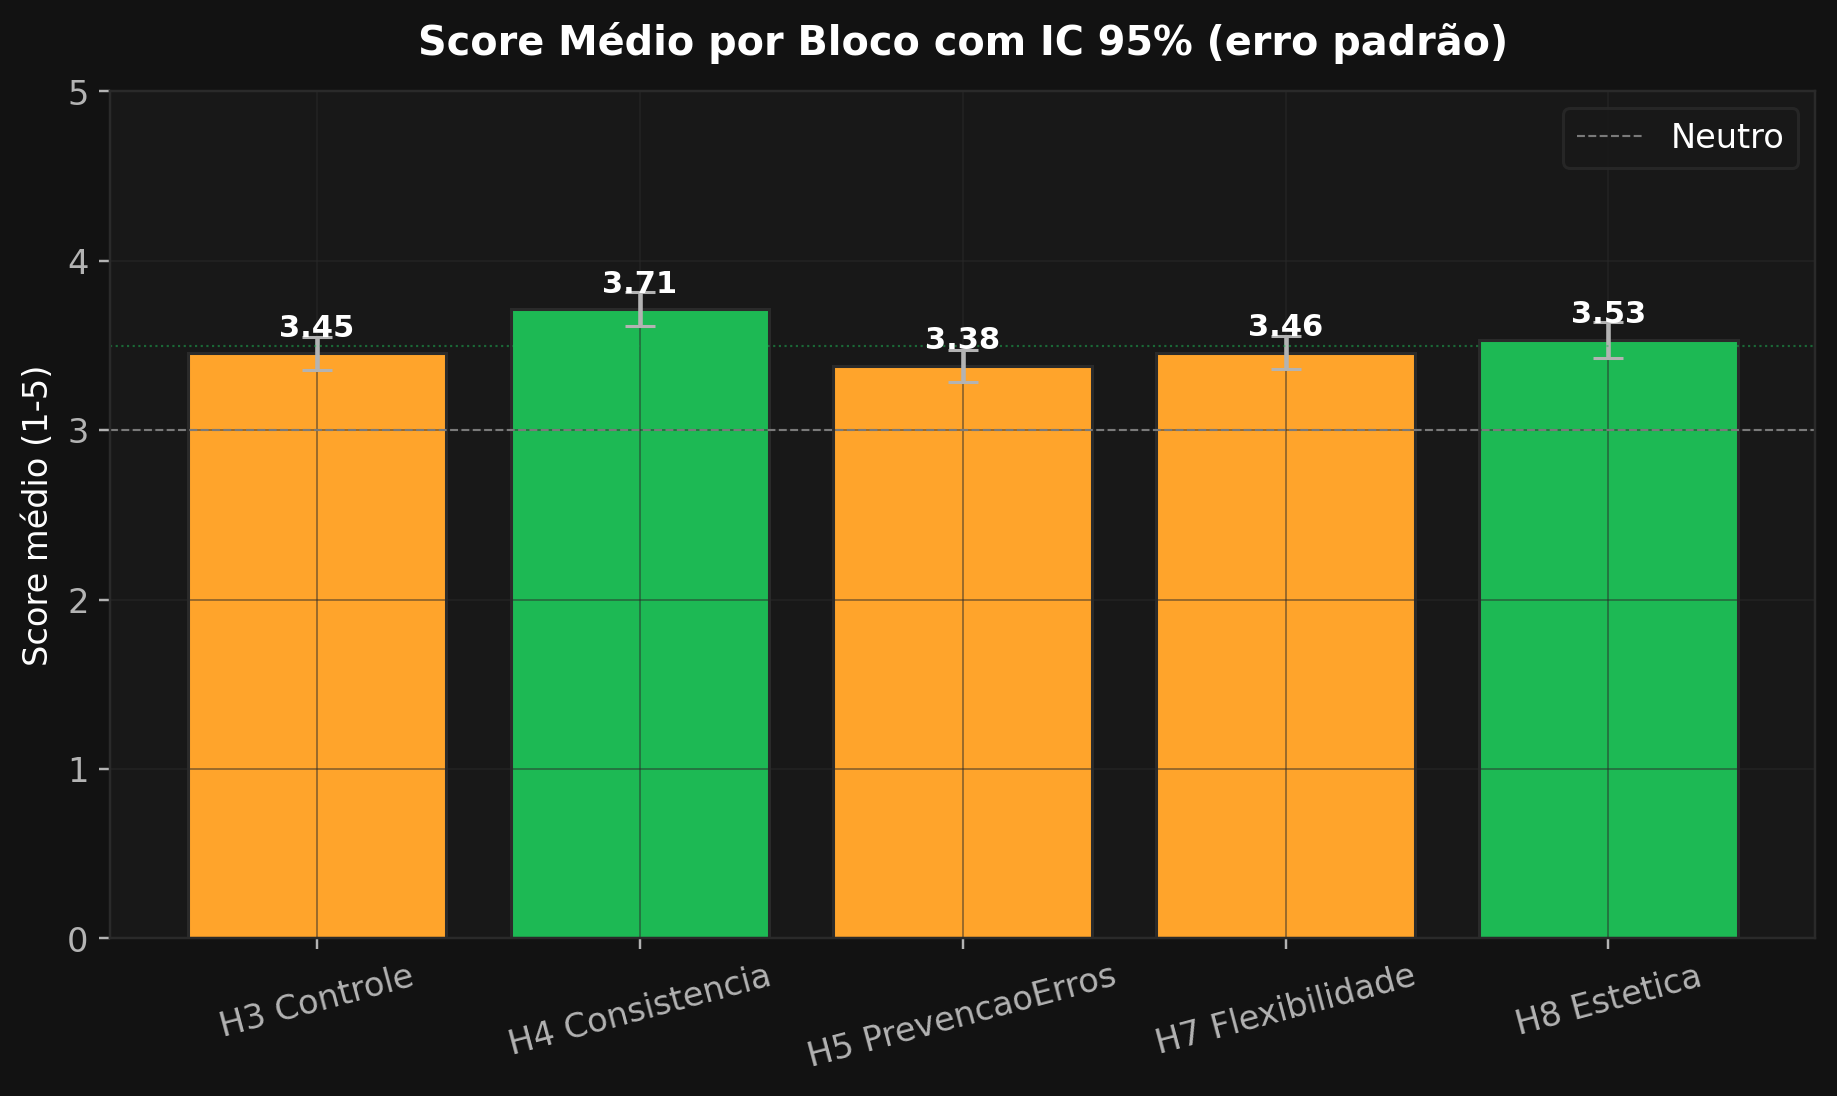
\includegraphics[width=0.82\linewidth]{figuras/fig10_score_blocos.png}
\caption{Score médio por bloco com erro padrão. Cores: verde $>3{,}5$;
âmbar $>3{,}0$; vermelho $\leq 3{,}0$.}
\label{fig:scores}
\end{figure}

\subsection{Estatística Descritiva por Bloco}
A Tabela~\ref{tab:desc-blocos} resume o score médio (média dos itens do bloco por
respondente) das cinco heurísticas avaliadas.

\begin{table}[h]
\centering
\caption{Estatística descritiva por bloco (heurística), $n = 86$.}
\label{tab:desc-blocos}
\small
\begin{tabular}{lrrrrr}
\toprule
\textbf{Bloco} & \textbf{Média} & \textbf{DP} & \textbf{Mediana}
& \textbf{\% Baixo $\leq$ 2{,}5} & \textbf{\% Alto $\geq$ 3{,}5}\\
\midrule
H4 --- Consistência         & \textbf{3{,}71} & 0{,}94 & 3{,}80 & 11{,}6\,\% & 62{,}8\,\%\\
H8 --- Estética/Minimalismo & 3{,}53          & 0{,}98 & 3{,}75 & 19{,}8\,\% & 59{,}3\,\%\\
H7 --- Flexibilidade        & 3{,}46          & 0{,}92 & 3{,}60 & 15{,}1\,\% & 53{,}5\,\%\\
H3 --- Controle/Liberdade   & 3{,}45          & 0{,}91 & 3{,}50 & 14{,}0\,\% & 52{,}3\,\%\\
H5 --- Prevenção de Erros   & \textbf{3{,}38} & 0{,}86 & 3{,}40 & 12{,}8\,\% & 47{,}7\,\%\\
\bottomrule
\end{tabular}
\end{table}

\textbf{Leitura.} Todos os blocos ficam acima do ponto neutro (3{,}0). O bloco mais bem
avaliado é H4 e o pior é H5 --- nenhum bloco está em zona de violação severa
no agregado. Esse achado \emph{contraria parcialmente} a expectativa do Trabalho~1 de
violações sistêmicas, e indica que as falhas residem em itens específicos, não em
dimensões inteiras.

A Figura~\ref{fig:netscore} apresenta o \textbf{Net Score} (\% Alto $-$ \% Baixo)
de cada item --- uma métrica única que sintetiza polaridade. Apenas \textbf{A3}
(\emph{desfazer playlist}) ficou negativo, com $-21{,}1$.

\begin{figure}[h]
\centering
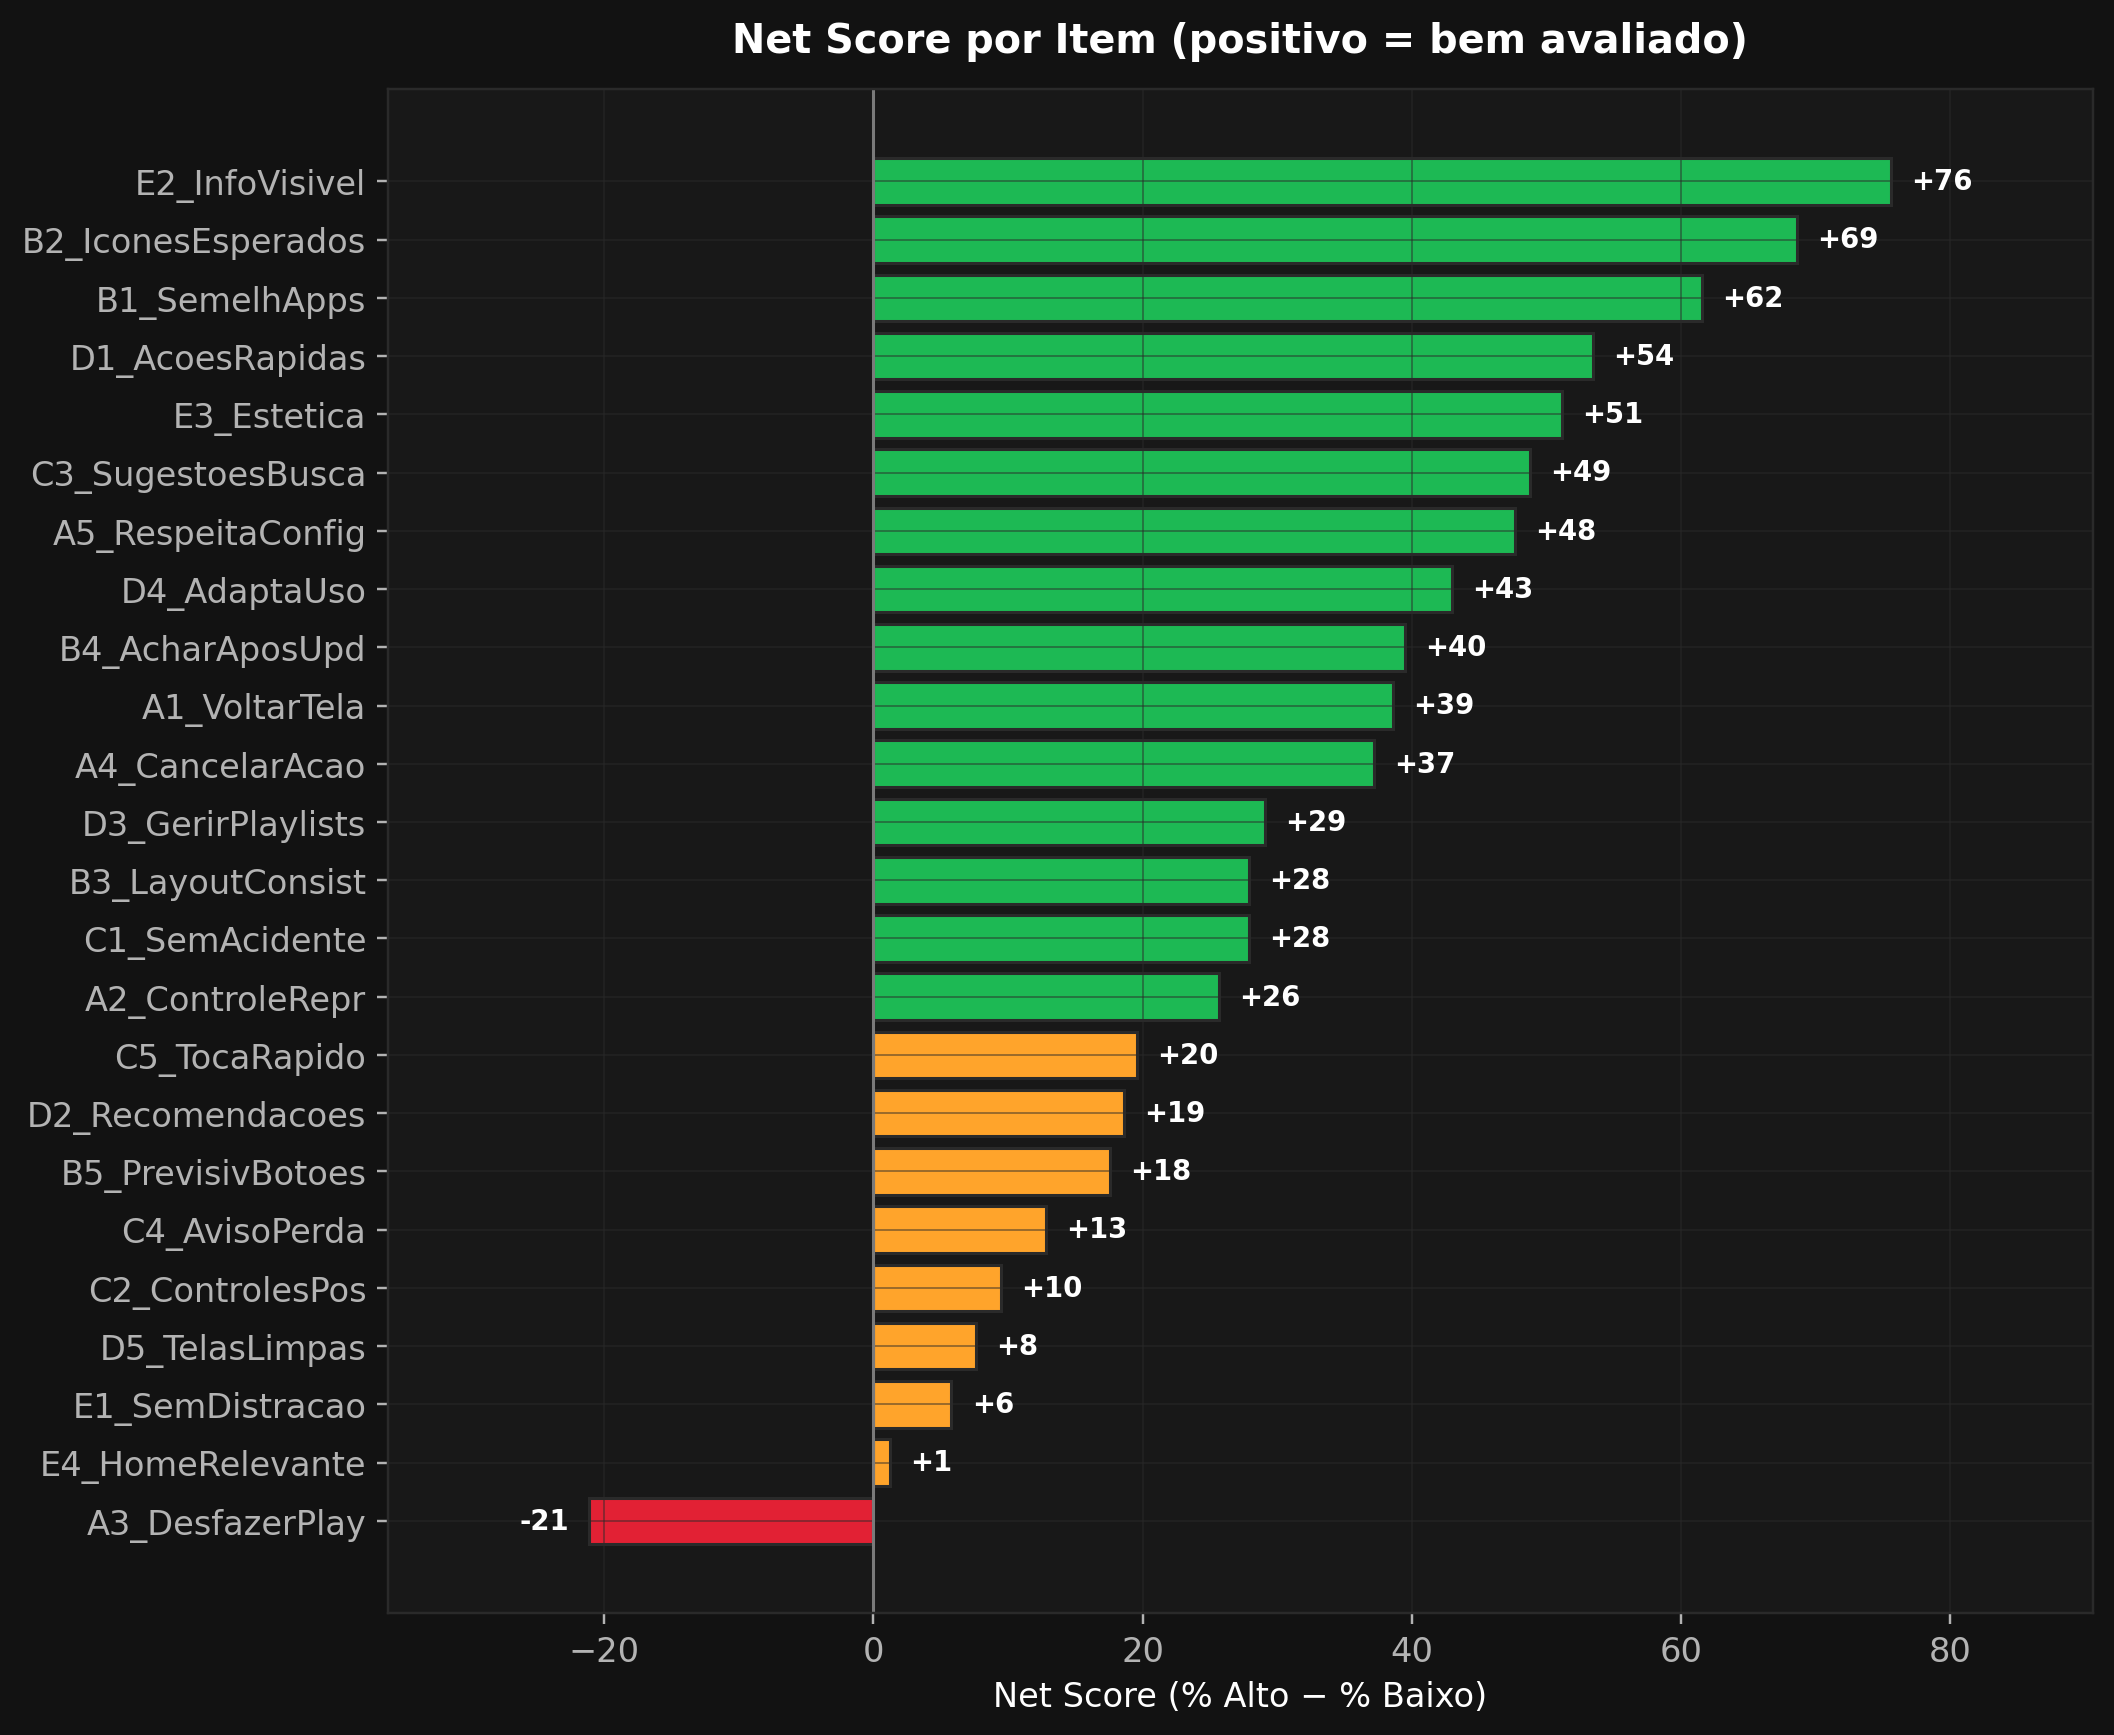
\includegraphics[width=0.85\linewidth]{figuras/fig3_net_score.png}
\caption{Net Score por item (\% Alto $-$ \% Baixo). A3 é o único item com Net negativo.}
\label{fig:netscore}
\end{figure}

\subsection{Itens críticos (pior desempenho)}
Os itens individuais com menor média e maior porcentagem de avaliações Baixas
(Tabela~\ref{tab:piores-itens}) revelam onde a usabilidade efetivamente falha.

\begin{table}[h]
\centering
\caption{Itens com pior desempenho ($n$ varia por item devido a \emph{NAs}).}
\label{tab:piores-itens}
\small
\begin{tabularx}{\linewidth}{l Y r r}
\toprule
\textbf{ID} & \textbf{Item} & \textbf{Média} & \textbf{\% Baixo}\\
\midrule
A3 & Desfazer adicionar/remover música em playlist (\textbf{H3}) & \textbf{2{,}58} & \textbf{46{,}5\,\%}\\
D5 & Telas livres de poluição (H7/H8)                            & 2{,}91         & 33{,}3\,\%\\
C2 & Posicionamento dos controles evita toque errado (H5)        & 2{,}92         & 28{,}6\,\%\\
E4 & Tela inicial relevante, sem promoções em excesso (\textbf{H8}) & \textbf{2{,}99} & \textbf{40{,}7\,\%}\\
B5 & Comportamento previsível dos botões (H4)                    & 3{,}06         & 27{,}5\,\%\\
E1 & Sem distrações (H8)                                         & 3{,}08         & 36{,}0\,\%\\
\bottomrule
\end{tabularx}
\end{table}

\subsection{Alpha de Cronbach}
Os valores de $\alpha$ avaliam a coesão interna do instrumento
(Tabela~\ref{tab:cronbach}).

\begin{table}[h]
\centering
\caption{Alpha de Cronbach por construto. Limiar do professor: $\alpha > 0{,}7$.}
\label{tab:cronbach}
\small
\begin{tabular}{lrrl}
\toprule
\textbf{Construto} & \textbf{$\alpha$} & \textbf{$n$ (listwise)} & \textbf{Interpretação}\\
\midrule
\textbf{Global (24 itens)}     & \textbf{0{,}961} & 18 & Excelente\\
H3 --- Controle                & 0{,}849          & 23 & Bom\\
H4 --- Consistência            & 0{,}785          & 51 & Aceitável\\
H5 --- Prevenção de Erros      & \textbf{0{,}672} & 46 & \textbf{Questionável}\\
H7 --- Flexibilidade           & 0{,}736          & 66 & Aceitável\\
H8 --- Estética                & 0{,}809          & 86 & Bom\\
\bottomrule
\end{tabular}
\end{table}

\textbf{Conclusões da confiabilidade:}
\begin{itemize}[leftmargin=*]
  \item Quatro dos cinco blocos atingem o limiar de aceitação;
  \item \textbf{H5 ficou em 0{,}672}, sugerindo que o construto ``Prevenção de Erros''
        não é totalmente coeso na redação atual; o item C5 (\emph{toca rapidamente})
        provavelmente mede mais \textbf{eficiência (H7)} do que prevenção, puxando o
        $\alpha$ para baixo;
  \item O $\alpha$ global de 0{,}961 (calculado em $n=18$ pelo \emph{listwise}) confirma
        que todos os itens medem coerentemente uma percepção única de
        \textbf{usabilidade do Spotify}.
\end{itemize}

\subsubsection*{Análise item-total (alpha-if-deleted)}
Para verificar quais itens individualmente sustentam o construto, calculamos a
correlação de cada item com o total do seu bloco (excluindo o próprio item) e
o $\alpha$ \emph{resultante caso o item seja removido}. A
Figura~\ref{fig:itemtotal} mostra a coesão item-bloco.

\begin{figure}[h]
\centering
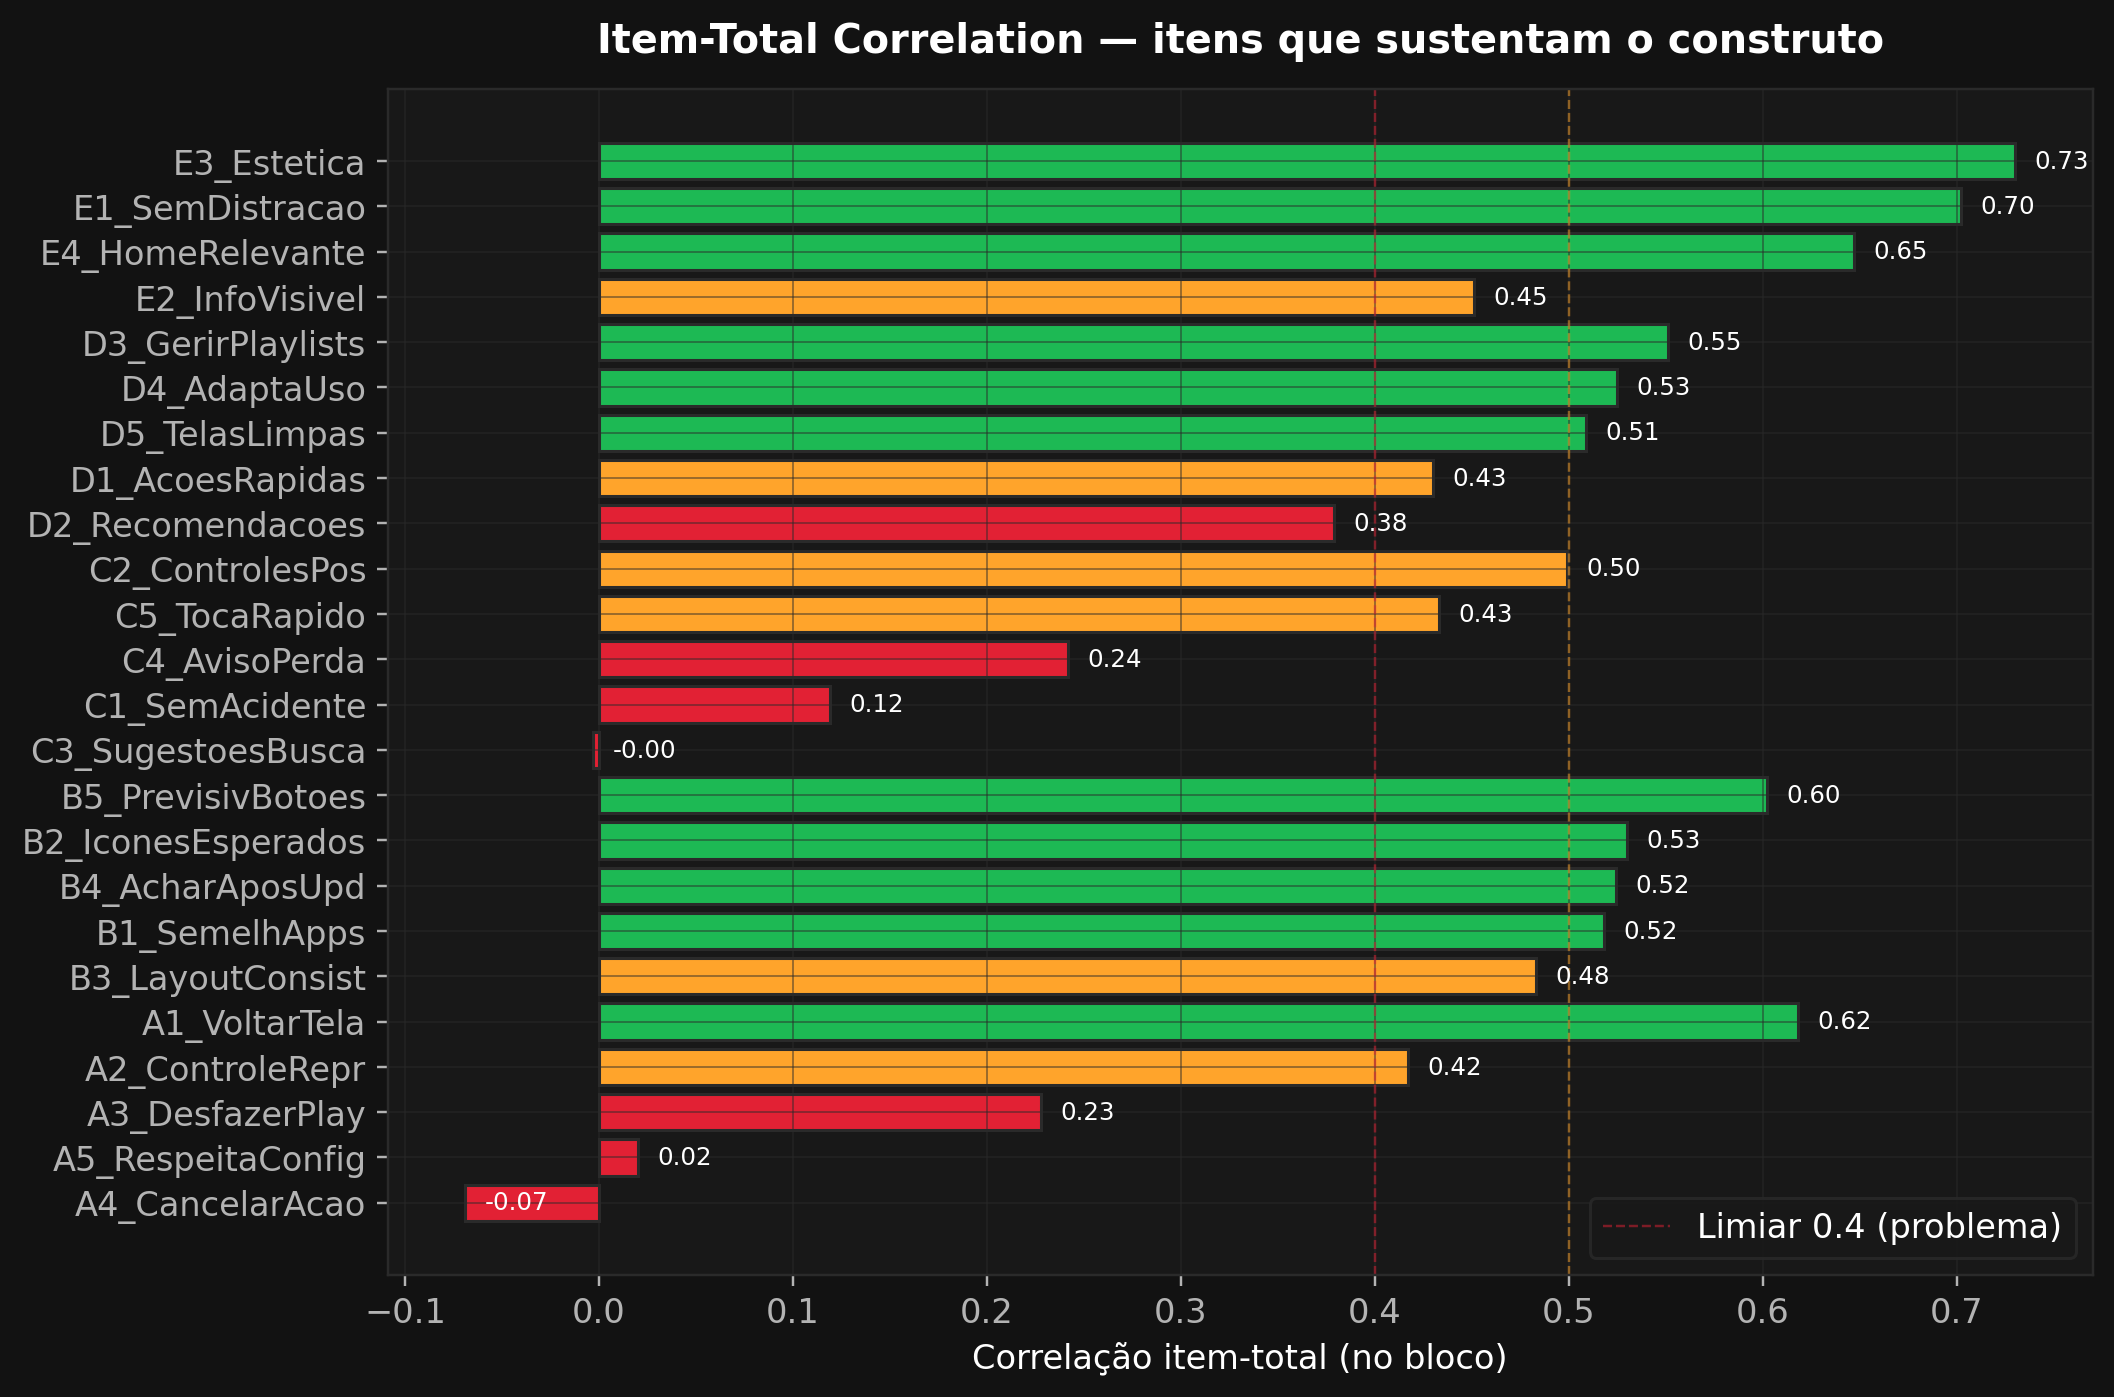
\includegraphics[width=0.85\linewidth]{figuras/fig8_item_total.png}
\caption{Correlação item-total por bloco. Vermelho: $r<0{,}4$ (item fraco);
âmbar: $0{,}4 \leq r < 0{,}5$; verde: $r \geq 0{,}5$.}
\label{fig:itemtotal}
\end{figure}

O item \textbf{C4 (\emph{Aviso de perda de dados})} tem $r_{\text{item-total}}=0{,}24$
no bloco H5 --- não compartilha variância suficiente com os demais. Este é o
principal responsável por $\alpha_{H5} = 0{,}67$. Recomenda-se reescrever o item
ou movê-lo para H3 (Controle/Liberdade) em iterações futuras do instrumento.

\subsection{Correlação de Pearson entre Blocos}
A matriz de correlação (Tabela~\ref{tab:corr-blocos}) explicita as relações entre as
cinco dimensões medidas.

\begin{table}[h]
\centering
\caption{Matriz de correlação de Pearson entre blocos ($pairwise.complete.obs$).}
\label{tab:corr-blocos}
\small
\begin{tabular}{lrrrrr}
\toprule
 & \textbf{H3} & \textbf{H4} & \textbf{H5} & \textbf{H7} & \textbf{H8}\\
\midrule
\textbf{H3 Controle}        & 1{,}000 & 0{,}691 & 0{,}560 & 0{,}640 & 0{,}693\\
\textbf{H4 Consistência}    & 0{,}691 & 1{,}000 & 0{,}691 & 0{,}718 & 0{,}714\\
\textbf{H5 Prev.\ Erros}    & 0{,}560 & 0{,}691 & 1{,}000 & 0{,}685 & 0{,}675\\
\textbf{H7 Flexibilidade}   & 0{,}640 & 0{,}718 & 0{,}685 & 1{,}000 & \textbf{0{,}802}\\
\textbf{H8 Estética}        & 0{,}693 & 0{,}714 & 0{,}675 & \textbf{0{,}802} & 1{,}000\\
\bottomrule
\end{tabular}
\end{table}

\textbf{Insight central:} \textbf{H7 (Flexibilidade) e H8 (Estética) caminham juntas com
$r = 0{,}802$ (forte)}. Usuários que percebem o app como visualmente limpo também o
percebem como eficiente para tarefas. Essa associação é a base estatística para a
hipótese central do redesign: \emph{reduzir poluição visual melhora a percepção de
eficiência}.

A Figura~\ref{fig:heatblocos} apresenta a matriz visualmente. Todas as
correlações entre blocos são moderadas a fortes ($r > 0{,}55$), reforçando que
as cinco heurísticas medem facetas de um construto único de \emph{usabilidade
percebida}.

\begin{figure}[h]
\centering
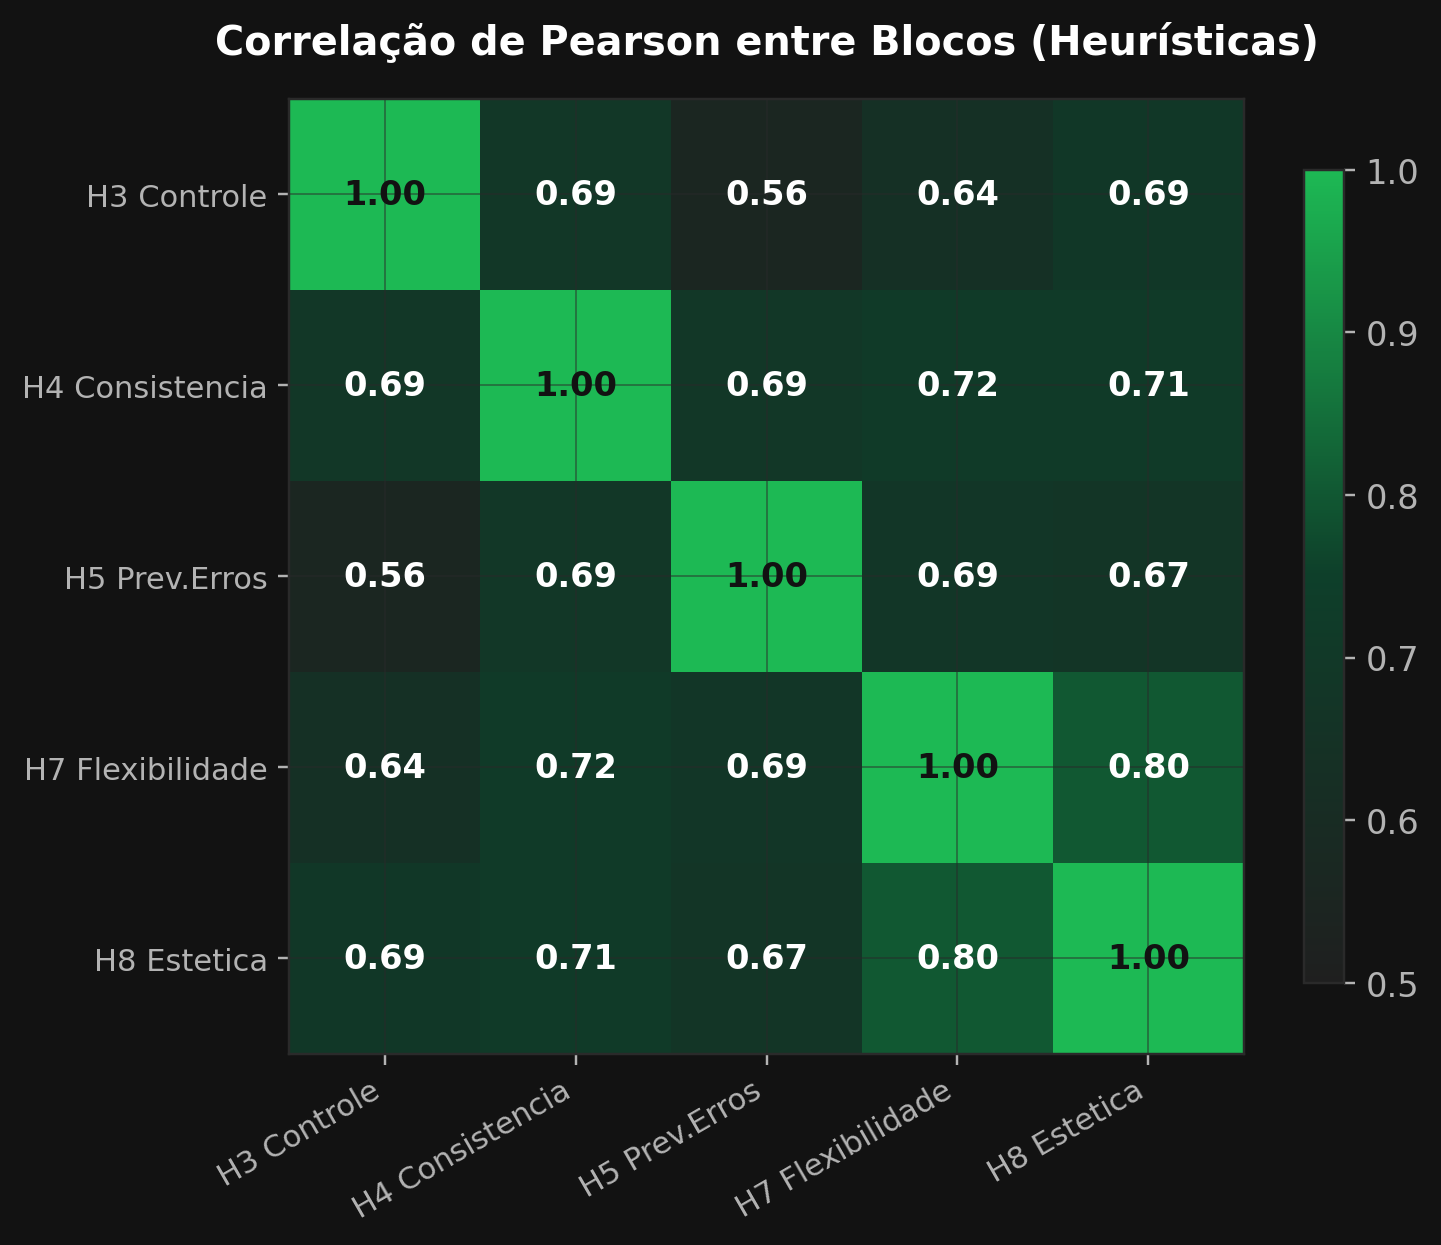
\includegraphics[width=0.55\linewidth]{figuras/fig2_heatmap_blocos.png}
\caption{Heatmap das correlações de Pearson entre blocos.}
\label{fig:heatblocos}
\end{figure}

\subsubsection*{Robustez: Spearman com correção de Bonferroni}
Como a escala Likert é \emph{ordinal} (não intervalar), repetimos a análise com
o coeficiente de Spearman e aplicamos a correção de Bonferroni para múltiplas
comparações ($m = 276$ pares item-item). Resultado: \textbf{88 dos 276 pares}
permanecem significativos com $p_{\text{corr}} < 0{,}05$, confirmando que as
associações encontradas \emph{não são artefato do tamanho amostral}.

A maior correlação de Spearman foi
\textbf{C2 (\emph{Controles bem posicionados}) $\leftrightarrow$ D5
(\emph{Telas limpas})} com $\rho = 0{,}77$, $p_{\text{Bonferroni}} = 6{,}4 \times 10^{-9}$
--- evidência muito forte do entrelaçamento entre layout e ergonomia de toque.

\subsection{Correlações item-a-item mais fortes ($|r| \geq 0{,}7$)}
\begin{table}[h]
\centering
\caption{Correlações fortes entre itens (top 5).}
\label{tab:corr-itens}
\small
\begin{tabularx}{\linewidth}{Y Y r}
\toprule
\textbf{Item A} & \textbf{Item B} & \textbf{r}\\
\midrule
A1 --- Voltar à tela anterior   & C5 --- Toca música rápido      & $+0{,}774$\\
B4 --- Achar após atualização   & C2 --- Controles bem posicion.\ & $+0{,}752$\\
C2 --- Controles bem posicion.\ & D5 --- Telas limpas            & $+0{,}750$\\
B3 --- Layout consistente       & E3 --- Estética agradável      & $+0{,}723$\\
A1 --- Voltar à tela anterior   & E2 --- Info importante visível & $+0{,}714$\\
\bottomrule
\end{tabularx}
\end{table}

\subsection{Regras de Associação (Apriori)}

\paragraph{Entre blocos} (suporte $\geq 0{,}10$ e confiança $\geq 0{,}60$ --- 90 regras
extraídas). As regras mais informativas estão na Tabela~\ref{tab:apriori-blocos}.

\begin{table}[h]
\centering
\caption{Top regras Apriori entre blocos (ordenadas por \emph{lift}).}
\label{tab:apriori-blocos}
\small
\begin{tabularx}{\linewidth}{Y r r r}
\toprule
\textbf{Regra (Se $\Rightarrow$ Então)} & \textbf{Sup} & \textbf{Conf} & \textbf{Lift}\\
\midrule
H4=\textbf{Baixo} $\Rightarrow$ H7=\textbf{Baixo} & 0{,}10 & \textbf{0{,}90} & \textbf{5{,}95}\\
H7=Baixo $\Rightarrow$ H4=Baixo                   & 0{,}10 & 0{,}69          & 5{,}95\\
H7=Baixo $\Rightarrow$ H8=Baixo                   & 0{,}12 & 0{,}77          & 3{,}89\\
H5=Alto $\wedge$ H8=Alto $\Rightarrow$ H7=Alto    & 0{,}36 & 0{,}91          & 1{,}70\\
H3=Alto $\wedge$ H8=Alto $\Rightarrow$ H7=Alto    & 0{,}35 & 0{,}86          & 1{,}60\\
\bottomrule
\end{tabularx}
\end{table}

\textbf{Achado de maior impacto.} A regra \textbf{H4=Baixo $\Rightarrow$ H7=Baixo}
($lift = 5{,}95$, confiança $90\,\%$) é a associação mais forte do estudo:
quando o usuário percebe inconsistência, é \emph{quase certo} (90\,\%) que
também percebe ineficiência. Esse é um argumento empírico direto contra
redesigns radicais que mudem layout sem migração progressiva.

A Figura~\ref{fig:apriori} visualiza as 1.030 regras-item no espaço
suporte~$\times$~confiança, coloridas por \emph{lift}.

\begin{figure}[h]
\centering
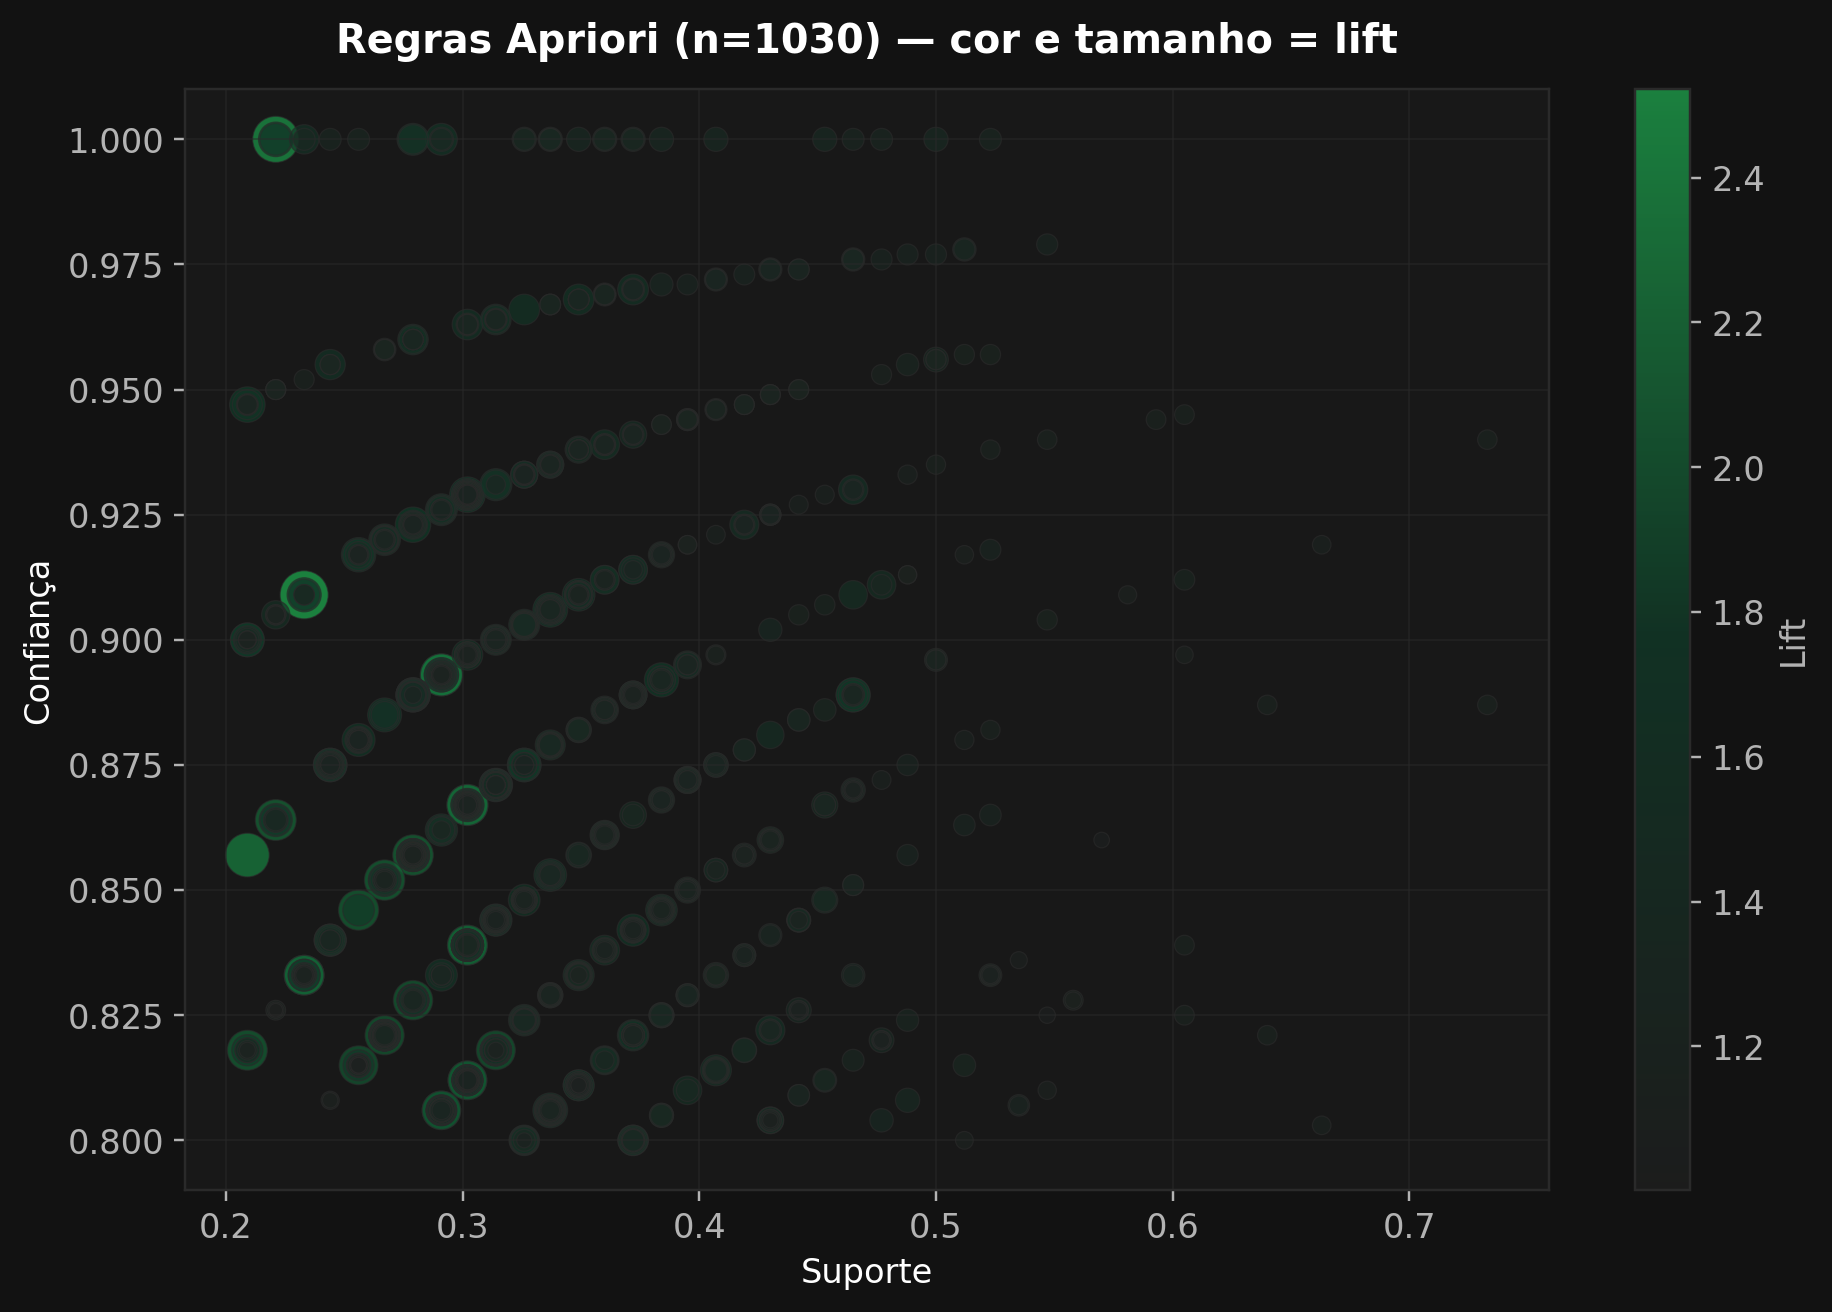
\includegraphics[width=0.85\linewidth]{figuras/fig5_apriori_scatter.png}
\caption{Regras Apriori entre itens. Tamanho e cor codificam o \emph{lift}.}
\label{fig:apriori}
\end{figure}

\subsection{Comparação Premium vs.\ Free}
\label{ssec:freevsprem}

Uma análise estratificada por tipo de conta revela uma \textbf{diferença
estatisticamente significativa em todos os cinco blocos}
(Tabela~\ref{tab:freeprem}). Aplicamos o teste não-paramétrico de
Mann-Whitney $U$, adequado para amostras pequenas e dados ordinais.

\begin{table}[h]
\centering
\caption{Score médio por bloco e teste de Mann-Whitney (Free vs.\ Premium).}
\label{tab:freeprem}
\small
\begin{tabular}{lrrrl}
\toprule
\textbf{Bloco} & \textbf{Free} (n=17) & \textbf{Premium} (n=69) & \textbf{$\Delta$} & \textbf{p} \\
\midrule
H3 --- Controle               & 2{,}83 & 3{,}61 & $+0{,}77$ & 0{,}0023 \textbf{(**)}\\
H4 --- Consistência           & 3{,}19 & 3{,}84 & $+0{,}66$ & 0{,}0464 (*)\\
H5 --- Prevenção de Erros     & 2{,}89 & 3{,}50 & $+0{,}61$ & 0{,}0345 (*)\\
H7 --- Flexibilidade          & 2{,}98 & 3{,}58 & $+0{,}60$ & 0{,}0251 (*)\\
H8 --- Estética               & 3{,}10 & 3{,}64 & $+0{,}54$ & 0{,}0268 (*)\\
\bottomrule
\end{tabular}
\end{table}

A Figura~\ref{fig:freevsprem} apresenta a comparação visualmente. Usuários do
plano \textbf{Free percebem o aplicativo entre 0{,}5 e 0{,}8 pontos abaixo}
dos usuários Premium em \emph{todas} as cinco heurísticas avaliadas. A maior
diferença ocorre em \textbf{H3 (Controle/Liberdade)} --- consistente com a
hipótese de que limitações artificiais do plano gratuito (não poder pular
músicas, modo aleatório forçado etc.) reduzem a sensação de controle.

\begin{figure}[h]
\centering
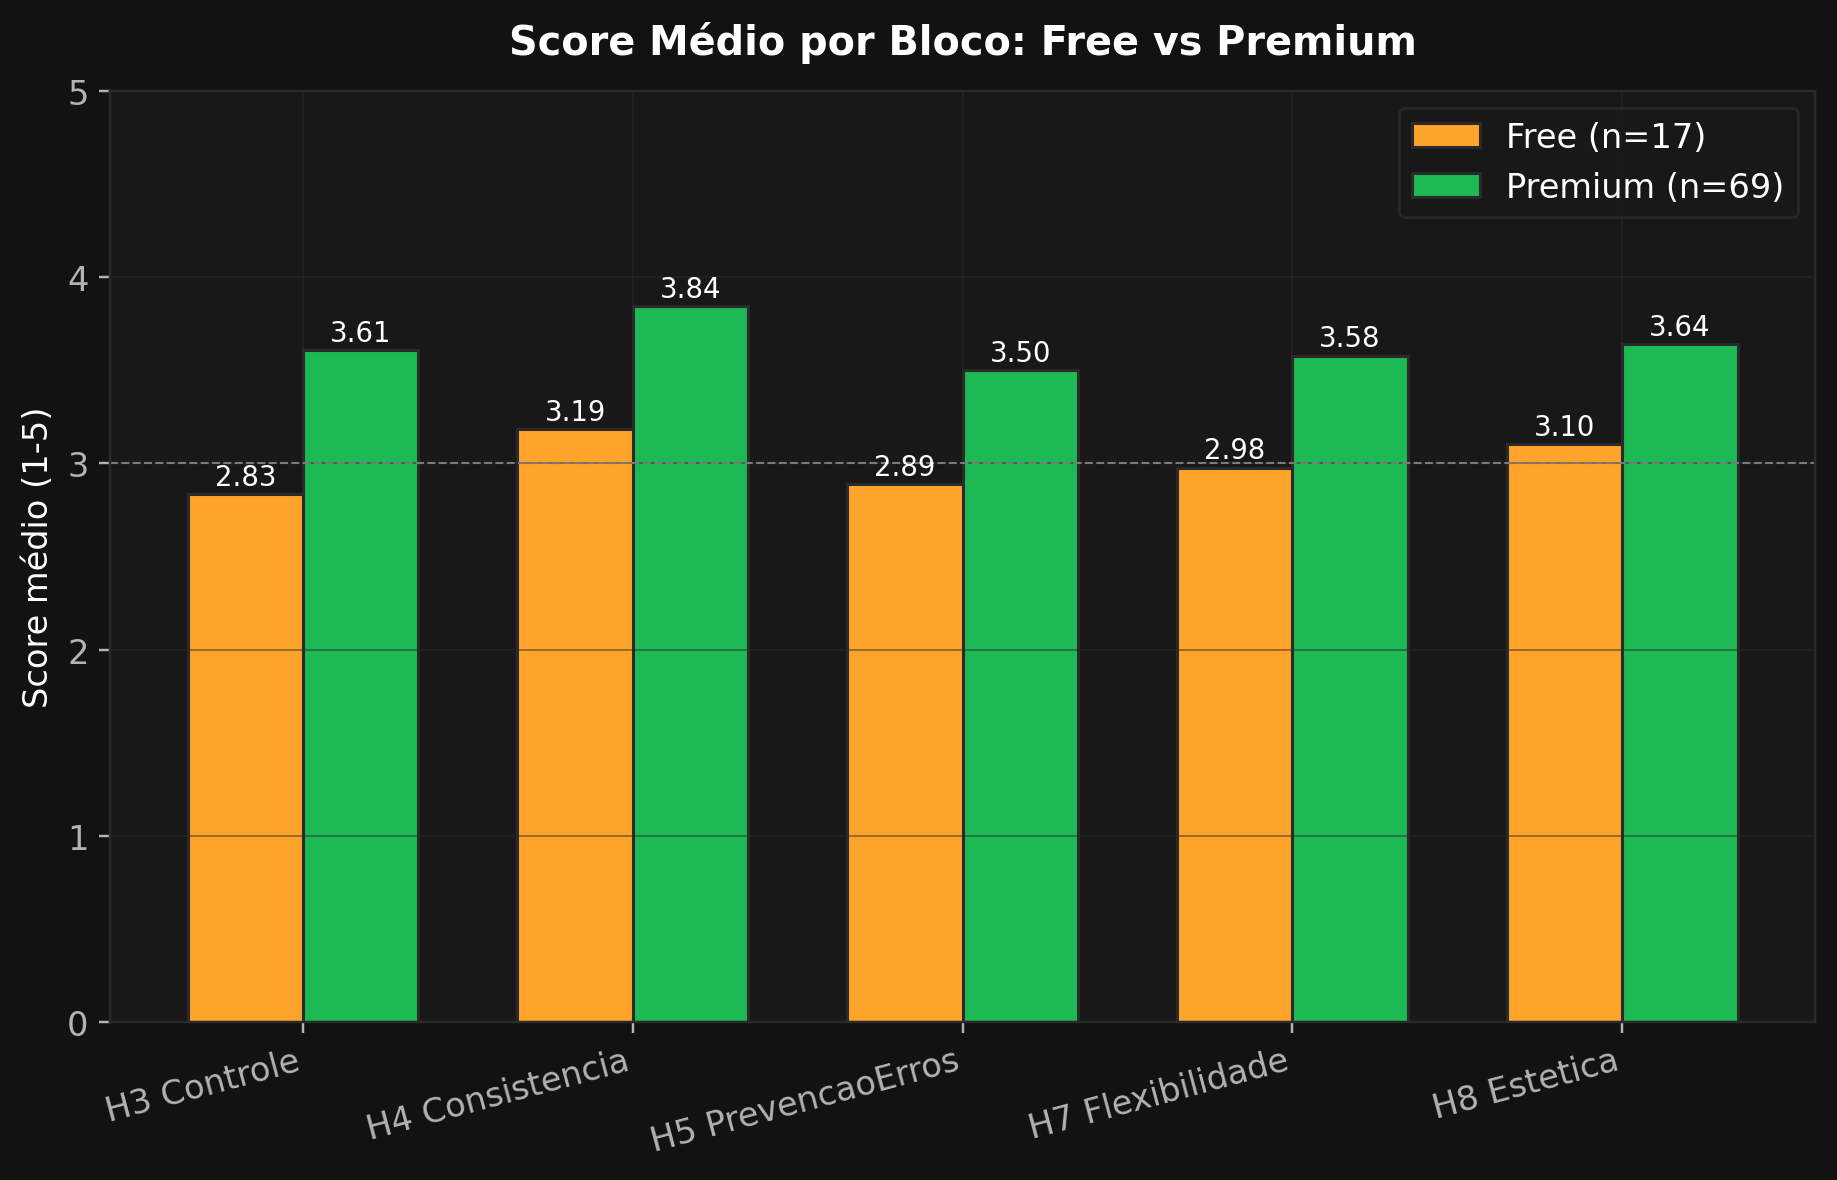
\includegraphics[width=0.82\linewidth]{figuras/fig6_free_vs_premium.png}
\caption{Score médio por bloco: Free (n=17) vs.\ Premium (n=69).}
\label{fig:freevsprem}
\end{figure}

\textbf{Implicação:} o problema não é apenas ``ter propaganda''. A monetização
freemium do Spotify degrada a usabilidade percebida em \textbf{todas as
dimensões}, não somente nas restrições visíveis. Isso é uma evidência fortíssima
de que o redesign deve incluir uma estratégia específica para a experiência Free.

\subsection{Qualidade dos Dados}
A análise de duração das respostas (Figura~\ref{fig:duracao}) mostra que:
\begin{itemize}[leftmargin=*]
  \item Mediana de resposta: $\approx$~502\,s ($\sim$8~min);
  \item Apenas \textbf{1 respondente (1{,}2\,\%)} levou menos de 2 minutos
        --- não há evidência de respondentes \emph{click-through};
  \item Quartis 25--75: 358\,s a 733\,s, intervalo coerente para um questionário
        de 24 itens Likert + 3 abertas.
\end{itemize}

\begin{figure}[h]
\centering
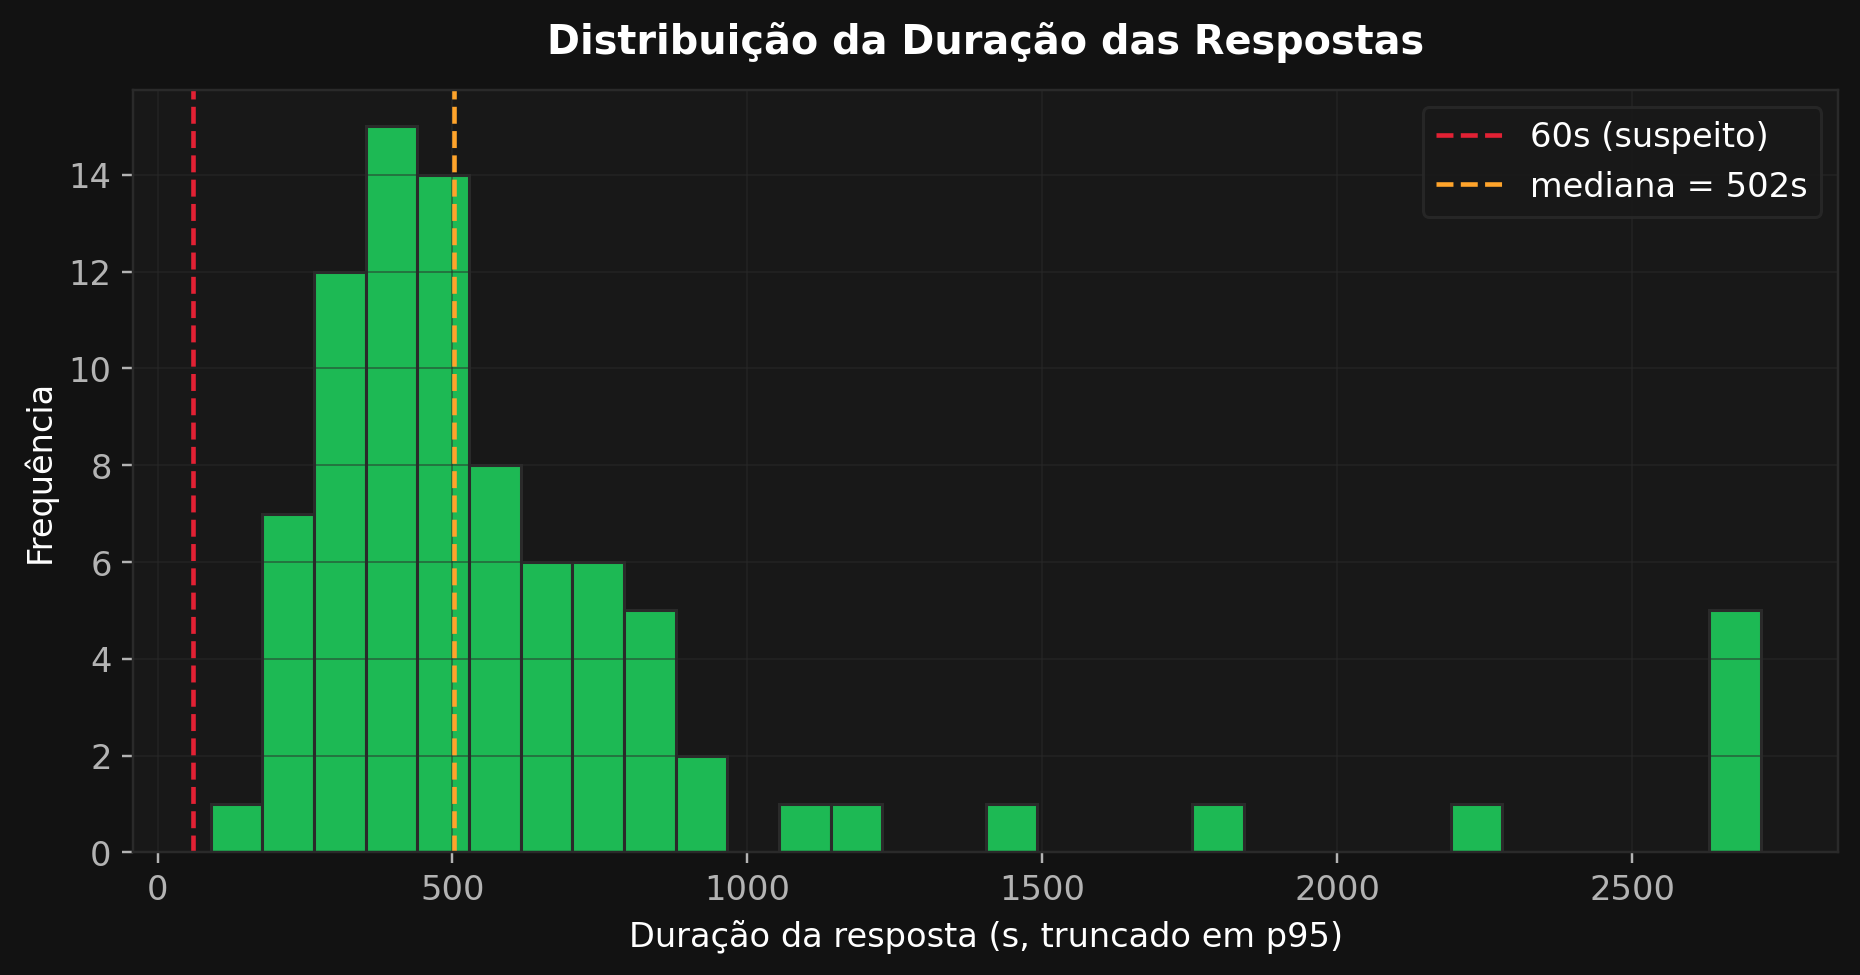
\includegraphics[width=0.78\linewidth]{figuras/fig7_duracao.png}
\caption{Distribuição da duração das respostas (truncada em $p_{95}$).}
\label{fig:duracao}
\end{figure}

\paragraph{Entre itens} (suporte $\geq 0{,}20$ e confiança $\geq 0{,}80$ --- 1.030 regras).
As mais notáveis estão na Tabela~\ref{tab:apriori-itens}.

\begin{table}[h]
\centering
\caption{Regras Apriori entre itens com maior impacto qualitativo.}
\label{tab:apriori-itens}
\small
\begin{tabularx}{\linewidth}{Y r r r}
\toprule
\textbf{Regra} & \textbf{Sup} & \textbf{Conf} & \textbf{Lift}\\
\midrule
D5 \emph{Telas limpas}=Baixo $\Rightarrow$ E1 \emph{Sem distrações}=Baixo  & 0{,}23 & 0{,}91 & 2{,}52\\
B3 \emph{Layout consist.}=Baixo $\Rightarrow$ A3 \emph{Desfazer playlist}=Baixo & 0{,}21 & 0{,}86 & 2{,}23\\
C4 \emph{Aviso perda}=Alto $\wedge$ E1=Alto $\Rightarrow$ E4 \emph{Home relevante}=Alto & 0{,}22 & 1{,}00 & 2{,}39\\
D5=Baixo $\Rightarrow$ E4 \emph{Home}=Baixo                                & 0{,}21 & 0{,}82 & 2{,}01\\
\bottomrule
\end{tabularx}
\end{table}

A regra \textbf{B3=Baixo $\Rightarrow$ A3=Baixo} ($lift = 2{,}23$) corrobora a hipótese
de que \textbf{a violação de H4 causa violação de H3}: layouts inconsistentes
provocam dificuldades em desfazer ações.

% =================== 4. ANÁLISE QUALITATIVA ===================
\section{Análise Qualitativa das Respostas Abertas}
\label{sec:qual}

Foram analisadas três perguntas abertas em 86 respostas. A codificação temática
mapeou cada menção à(s) heurística(s) violada(s) ou a temas externos
(modelo de negócio e performance). A Tabela~\ref{tab:qual} e a
Figura~\ref{fig:pareto} resumem a distribuição via diagrama de Pareto.

\begin{figure}[h]
\centering
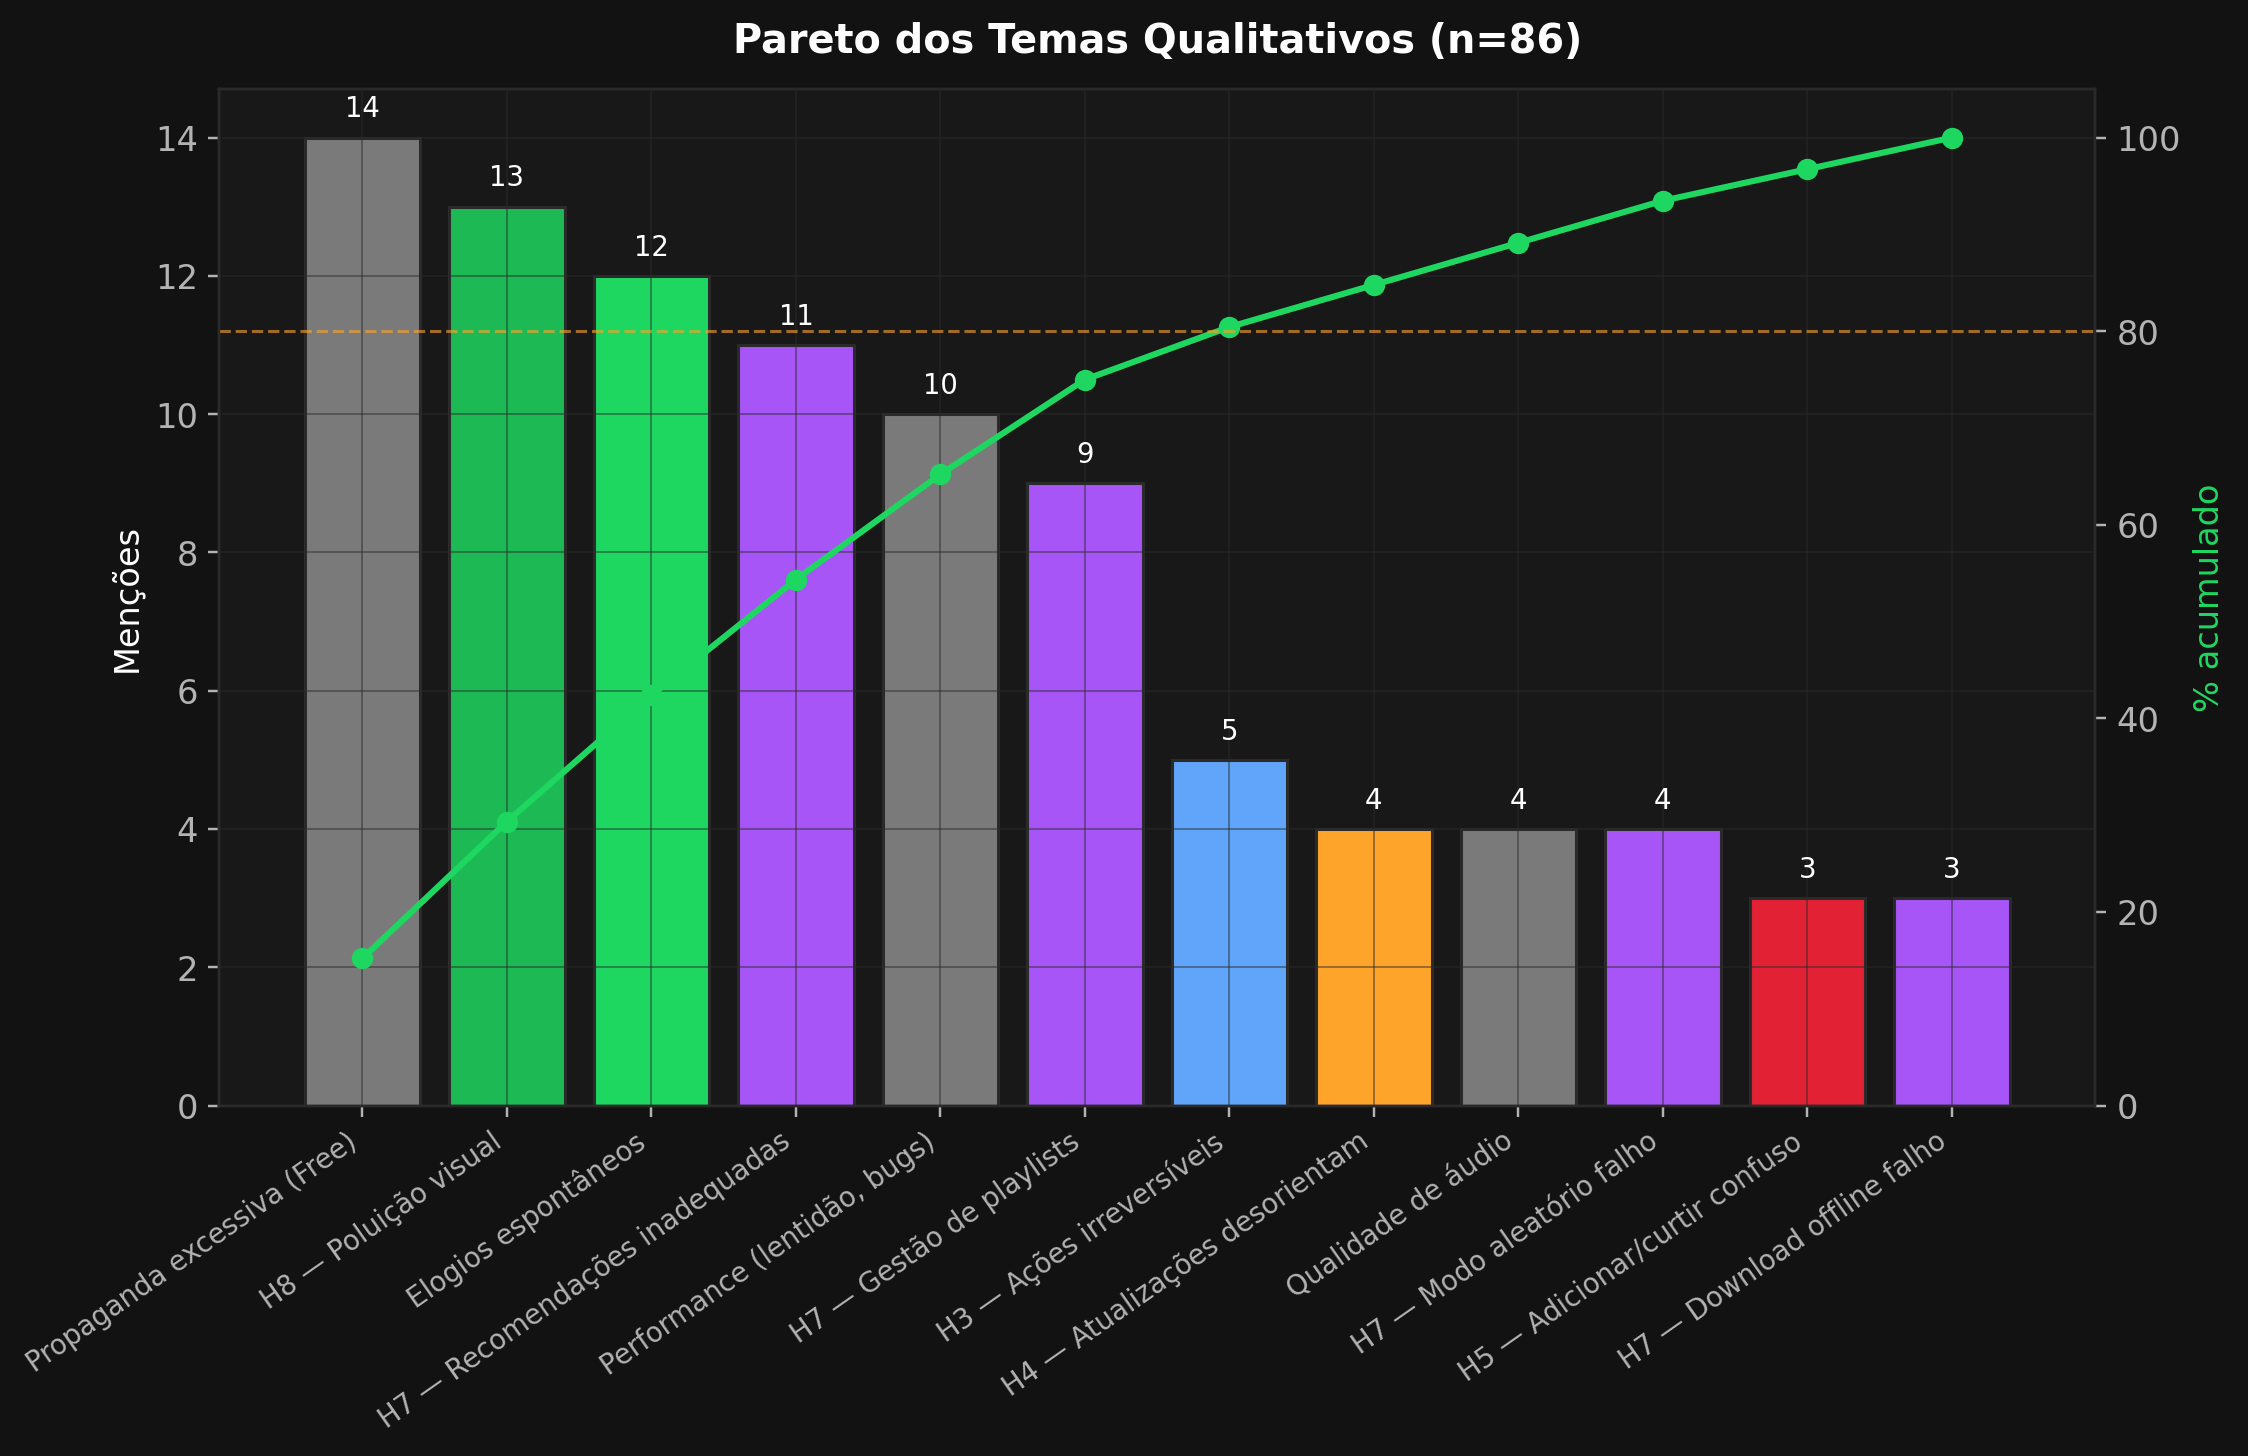
\includegraphics[width=0.92\linewidth]{figuras/fig4_pareto_qualitativo.png}
\caption{Diagrama de Pareto dos temas qualitativos. A linha laranja marca
80\,\% acumulado. Cinco temas concentram $\sim$70\,\% das menções.}
\label{fig:pareto}
\end{figure}

\begin{table}[h]
\centering
\caption{Distribuição das menções por tema (codificação qualitativa).}
\label{tab:qual}
\small
\begin{tabularx}{\linewidth}{Y r r}
\toprule
\textbf{Tema} & \textbf{Menções} & \textbf{\% válidos}\\
\midrule
Excesso de propaganda no plano Free                 & 14 & 16{,}3\,\%\\
\textbf{H8 --- Poluição visual / excesso de informação} & \textbf{13} & 15{,}1\,\%\\
\textbf{H7 --- Recomendações inadequadas}           & \textbf{11} & 12{,}8\,\%\\
Performance (travamentos, lentidão, bugs)           & 10 & 11{,}6\,\%\\
\textbf{H7 --- Gestão ineficiente de playlists/biblioteca} & 9 & 10{,}5\,\%\\
\textbf{H3 --- Ações irreversíveis} (apagar, fechar busca) & 5 & 5{,}8\,\%\\
\textbf{H4 --- Atualizações de UI desorientam}      & 4 & 4{,}7\,\%\\
Qualidade de áudio / compressão                     & 4 & 4{,}7\,\%\\
Elogios espontâneos                                  & 12 & 14{,}0\,\%\\
\bottomrule
\end{tabularx}
\end{table}

\subsection{Citações representativas (com identificador)}
\begin{description}[leftmargin=2cm, style=nextline]
  \item[\textbf{H3 (Controle)}] ``Já limpei sem querer a barra de pesquisa e não
       consegui reverter.'' --- \emph{E51}.
  \item[\textbf{H3 (Controle)}] ``Apenas algumas operações que não podem ser desfeitas,
       como apagar música de playlist; se eu apagasse uma música, aparecesse um pop-up
       para poder reverter.'' --- \emph{E83}.
  \item[\textbf{H4 (Consistência)}] ``Não conseguia encontrar meus artistas salvos,
       após uma atualização de overhaul do visual.'' --- \emph{E02}.
  \item[\textbf{H4 (Consistência)}] ``Confusão principalmente quando o aplicativo muda
       o layout ou algumas funções de lugar.'' --- \emph{E59}.
  \item[\textbf{H5 (Prevenção)}] ``Quando tento adicionar uma música na playlist mas
       ela é salva nas músicas curtidas.'' --- \emph{E08}.
  \item[\textbf{H7 (Flexibilidade)}] ``Não ter como transferir músicas de uma playlist
       para a outra facilmente, tem q fazer uma a uma.'' --- \emph{E03}.
  \item[\textbf{H8 (Estética)}] ``Deixaria o Spotify mais limpo. São muitas informações
       desnecessárias, propagandas e coisas que não me agregam em nada.'' --- \emph{E19}.
  \item[\textbf{H8 (Estética)}] ``Layout poluído, com muitas vezes informações
       desnecessárias e playlists não usuais.'' --- \emph{E51}.
\end{description}

% =================== 5. DISCUSSÃO ===================
\section{Discussão das Evidências}
\label{sec:discussao}

A Tabela~\ref{tab:vereditos} cruza, para cada hipótese do Trabalho~1, o score do bloco,
o $\alpha$ correspondente, a evidência qualitativa e o veredito final.

\begin{table}[h]
\centering
\caption{Vereditos das hipóteses do Trabalho 1 à luz dos resultados.}
\label{tab:vereditos}
\footnotesize
\begin{tabularx}{\linewidth}{l r r Y l}
\toprule
\textbf{Hipótese} & \textbf{Média} & \textbf{$\alpha$} & \textbf{Evidência qualitativa} & \textbf{Veredito}\\
\midrule
H3 Controle/Liberdade   & 3{,}45 & 0{,}85 & 5 menções; A3 com 46{,}5\,\% baixo & \textbf{Parcial} (item)\\
H4 Consistência         & 3{,}71 & 0{,}79 & 4 menções (atualizações) & Não confirmada (agregado)\\
H5 Prevenção de Erros   & 3{,}38 & \textbf{0{,}67} & 3 menções; bloco mais fraco & \textbf{Parcial}\\
H7 Flexibilidade/Eficiência & 3{,}46 & 0{,}74 & 11+9 menções & \textbf{Confirmada}\\
H8 Estética/Minimalismo & 3{,}53 & 0{,}81 & 13 menções; E4 e E1 muito baixos & \textbf{Confirmada}\\
\bottomrule
\end{tabularx}
\end{table}

\subsection*{Síntese das evidências}
\begin{enumerate}[leftmargin=*, itemsep=2pt]
  \item \textbf{H7 e H8 são confirmadas robustamente} --- correlação forte ($r=0{,}802$),
        regras Apriori convergentes e o maior volume de menções qualitativas
        (24~no total). É a evidência mais sólida do estudo.
  \item \textbf{H3 confirma-se pontualmente, não no bloco} --- o item \textbf{A3}
        (\emph{desfazer ações em playlist}) com média 2{,}58 e 46{,}5\,\% baixo é o pior
        item de todo o questionário, reforçado por relatos diretos (E51, E83).
  \item \textbf{H5 é a mais frágil estatisticamente} ($\alpha = 0{,}67$). Sugere
        revisão do construto: itens como C5 (\emph{toca rápido}) podem migrar
        para H7. Ainda assim, o problema concreto de ``curtir vs.\ adicionar a
        playlist'' (E08, E13) está documentado.
  \item \textbf{H4 só falha quando o app muda} --- o agregado é positivo (3{,}71), mas
        \emph{atualizações de UI desorientam} usuários veteranos (E02, E20, E59).
  \item \textbf{Tema externo dominante:} \emph{excesso de propaganda no Free} (16{,}3\,\%
        das menções) lidera os comentários, mas é uma decisão de \emph{modelo de
        negócio}, não de usabilidade clássica.
\end{enumerate}

% =================== 6. RECOMENDAÇÕES ===================
\section{Conclusão e Recomendações para o Protótipo}
\label{sec:conclusao}

A análise integrada dos dados quantitativos e qualitativos converge para
\textbf{seis recomendações de redesign priorizadas por evidência empírica}, mostradas
na Tabela~\ref{tab:proto}.

\begin{table}[h]
\centering
\caption{Recomendações para o protótipo de melhoria (priorizadas por evidência).}
\label{tab:proto}
\footnotesize
\begin{tabularx}{\linewidth}{c Y Y c}
\toprule
\textbf{\#} & \textbf{Mudança proposta} & \textbf{Justificativa empírica} & \textbf{Esforço}\\
\midrule
1 & \textbf{Snackbar ``Desfazer'' persistente em ações de playlist} &
    A3 = 2{,}58 (pior item); 46{,}5\,\% baixo; E51/E83 & Baixo\\
2 & \textbf{Modo ``Home minimalista''} (ocultar promoções e \emph{podcasts}
    sugeridos pré-instalados) &
    E4 = 2{,}99 (40{,}7\,\% baixo); 13 menções; D5$\Rightarrow$E4 lift~2{,}01 & Médio\\
3 & \textbf{Separar visualmente ``Curtir'' de ``Adicionar a playlist''} (botões distintos) &
    Bloco H5 com pior $\alpha$ e média; relatos E08, E13 & Baixo\\
4 & \textbf{Seleção múltipla em playlists} (mover/remover em lote) &
    H7 com 9 menções; E03, E51, E86 & Médio\\
5 & \textbf{Migração progressiva em redesigns} (\emph{coach marks}, opção
    ``manter layout antigo'' por 30 dias) &
    H4$\Rightarrow$H7 lift~5{,}95; E02, E20, E59 & Alto\\
6 & \textbf{Indicação visual mais firme de configurações persistentes}
    (ex.: shuffle desativado fica desativado) &
    A5 = 3{,}79 mas itens H5 fracos; relato E35 & Baixo\\
7 & \textbf{Repensar onboarding e UX específico do plano Free} &
    Free $0{,}5$--$0{,}8$ abaixo em \emph{todos} os blocos
    (Mann-Whitney $p < 0{,}05$ em 5/5); 14 menções a propaganda. \S\ref{ssec:freevsprem}.
    & Estratégico\\
\bottomrule
\end{tabularx}
\end{table}

\subsection*{Princípios de redesign destilados das evidências}
\begin{itemize}[leftmargin=*]
  \item \textbf{Menos é mais (H8 + H7).} A correlação forte entre ``telas limpas''
        e ``eficiência percebida'' ($r = 0{,}802$) indica que \textbf{toda redução de
        ruído visual paga dividendos duplos}: melhora estética \emph{e} produtividade
        percebida.
  \item \textbf{Reversibilidade radical (H3).} Toda ação destrutiva em playlist
        precisa ter um caminho de retorno explícito, sem custo cognitivo. O usuário
        precisa sentir confiança para experimentar.
  \item \textbf{Estabilidade da forma (H4 $\to$ H7).} A regra Apriori
        H4=Baixo $\Rightarrow$ H7=Baixo (\emph{lift} 5{,}95) implica que mudanças
        de layout, mesmo bem-intencionadas, têm custo alto para usuários experientes.
        Redesigns devem ser \emph{opt-in} ou progressivos.
  \item \textbf{Foco em alvos específicos, não em blocos inteiros.} Como nenhuma
        heurística está integralmente reprovada no agregado, o redesign deve ser
        cirúrgico --- atacar A3, E4, E1 e D5 antes de qualquer reformulação geral.
\end{itemize}

\subsection*{Limitações e próximos passos}
\begin{itemize}[leftmargin=*]
  \item Amostra enviesada para usuários jovens, universitários e \emph{Premium}
        ($n=86$). Resultados são robustos para esse perfil; uma expansão para o
        público Free e para faixas etárias 35+ é desejável.
  \item $\alpha$ de H5 abaixo de 0{,}7 sinaliza necessidade de reescrever os itens
        do bloco em versões futuras do instrumento.
  \item Discretização Likert$\to$Alto/Neutro/Baixo para Apriori é uma simplificação
        que perde granularidade ordinal --- útil para regras qualitativas, não para
        inferência fina.
  \item A próxima etapa do projeto (Trabalho 3) consolida estas seis recomendações
        em um \textbf{protótipo de alta fidelidade} a ser avaliado em laboratório
        (Território n.\,14).
\end{itemize}

% =================== ANEXO ===================
\appendix
\section{Anexos}

\subsection{Estrutura de Arquivos da Análise}
Todos os arquivos estão em \texttt{docs/analise/}:

\begin{itemize}[leftmargin=*, itemsep=1pt]
  \item \texttt{analise.py} --- pipeline Python (\emph{executado}).
  \item \texttt{analise.R} --- versão R equivalente (espelha o \texttt{exemplo.R}).
  \item \texttt{dados.csv} --- 86 respondentes $\times$ 30 variáveis (sep.\ ``;'').
  \item \texttt{respostas\_abertas.csv} --- Q33/Q34/Q35 + demografia.
  \item \texttt{saida\_descritiva\_itens.csv} --- média, DP, \% por item.
  \item \texttt{saida\_descritiva\_blocos.csv} --- estatísticas por heurística.
  \item \texttt{saida\_corr\_blocos.csv} --- matriz Pearson 5$\times$5.
  \item \texttt{saida\_corr\_fortes.csv} --- correlações item-item com $|r| \geq 0{,}5$.
  \item \texttt{saida\_apriori\_blocos.csv} --- 90 regras (nível bloco).
  \item \texttt{saida\_apriori\_itens.csv} --- 1.030 regras (nível item).
  \item \texttt{saida\_log.txt} --- log completo de execução.
  \item \texttt{saida\_resumo.json} --- resumo programático para reuso.
  \item \texttt{codificacao\_qualitativa.md} --- codificação das abertas.
  \item \texttt{RELATORIO\_ANALISE.md} --- versão Markdown deste relatório.
  \item \texttt{relatorio.tex} / \texttt{relatorio.pdf} --- este documento.
\end{itemize}

\subsection{Reprodutibilidade}
Para reexecutar a análise:

\begin{lstlisting}[style=pystyle, caption={Comando de execução.}]
cd docs/analise/
python3 analise.py    # gera todas as saidas saida_*.csv|json
\end{lstlisting}

A versão R (\texttt{analise.R}), espelhando o \texttt{exemplo.R} do professor,
está disponível para auditoria.

\end{document}
